%-------------------------------------------------------------------------------
\begin{frame}
  \frametitle{Stratégie pour la résolution du problème}
  Plusieurs stratégie possible:
  \begin{itemize}
    \item Méthode intégrale (Choix Axessim)
    \item Méthode élément finis
    \begin{itemize}
    \item Découplage du problème en sous problème simple (Nécessite
      un réassemblage des sous-matrices L et de générer le découpage du maillage).
    \item Résolution du système complet (FreeFEM, Feel++).
    \end{itemize}
  \end{itemize}
\end{frame}
%-------------------------------------------------------------------------------

%-------------------------------------------------------------------------------
\begin{frame}
  \frametitle{G\'en\'eration de conducteurs et maillage}
  \begin{columns}[T]
    \column{.5\linewidth}
    \begin{itemize}
      \item Maillage explicite sur des cas tests simples.
      \item G\'en\'eralisation sur des g\'eom\'etrie contenant des conducteurs
        imbriqu\'e sur diff\'erent niveaux (blindages successifs).
      \item Utilisation d'outils de maillage automatique et param\'etrique (GMSH et FreeFem)
    \end{itemize}
    \column{.5\linewidth}
    \centering
    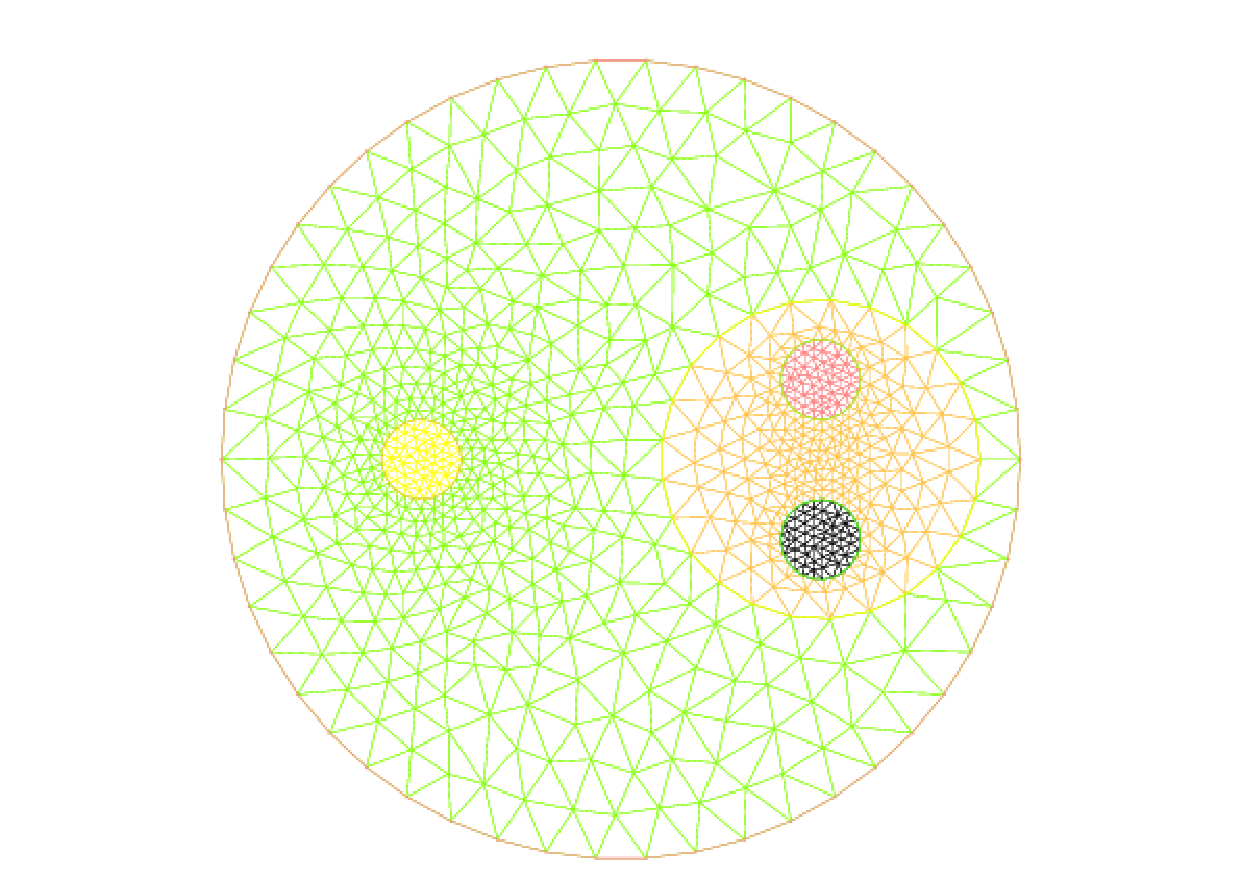
\includegraphics[width=.7\linewidth]{figures/gui/mesh-1.pdf}\\
    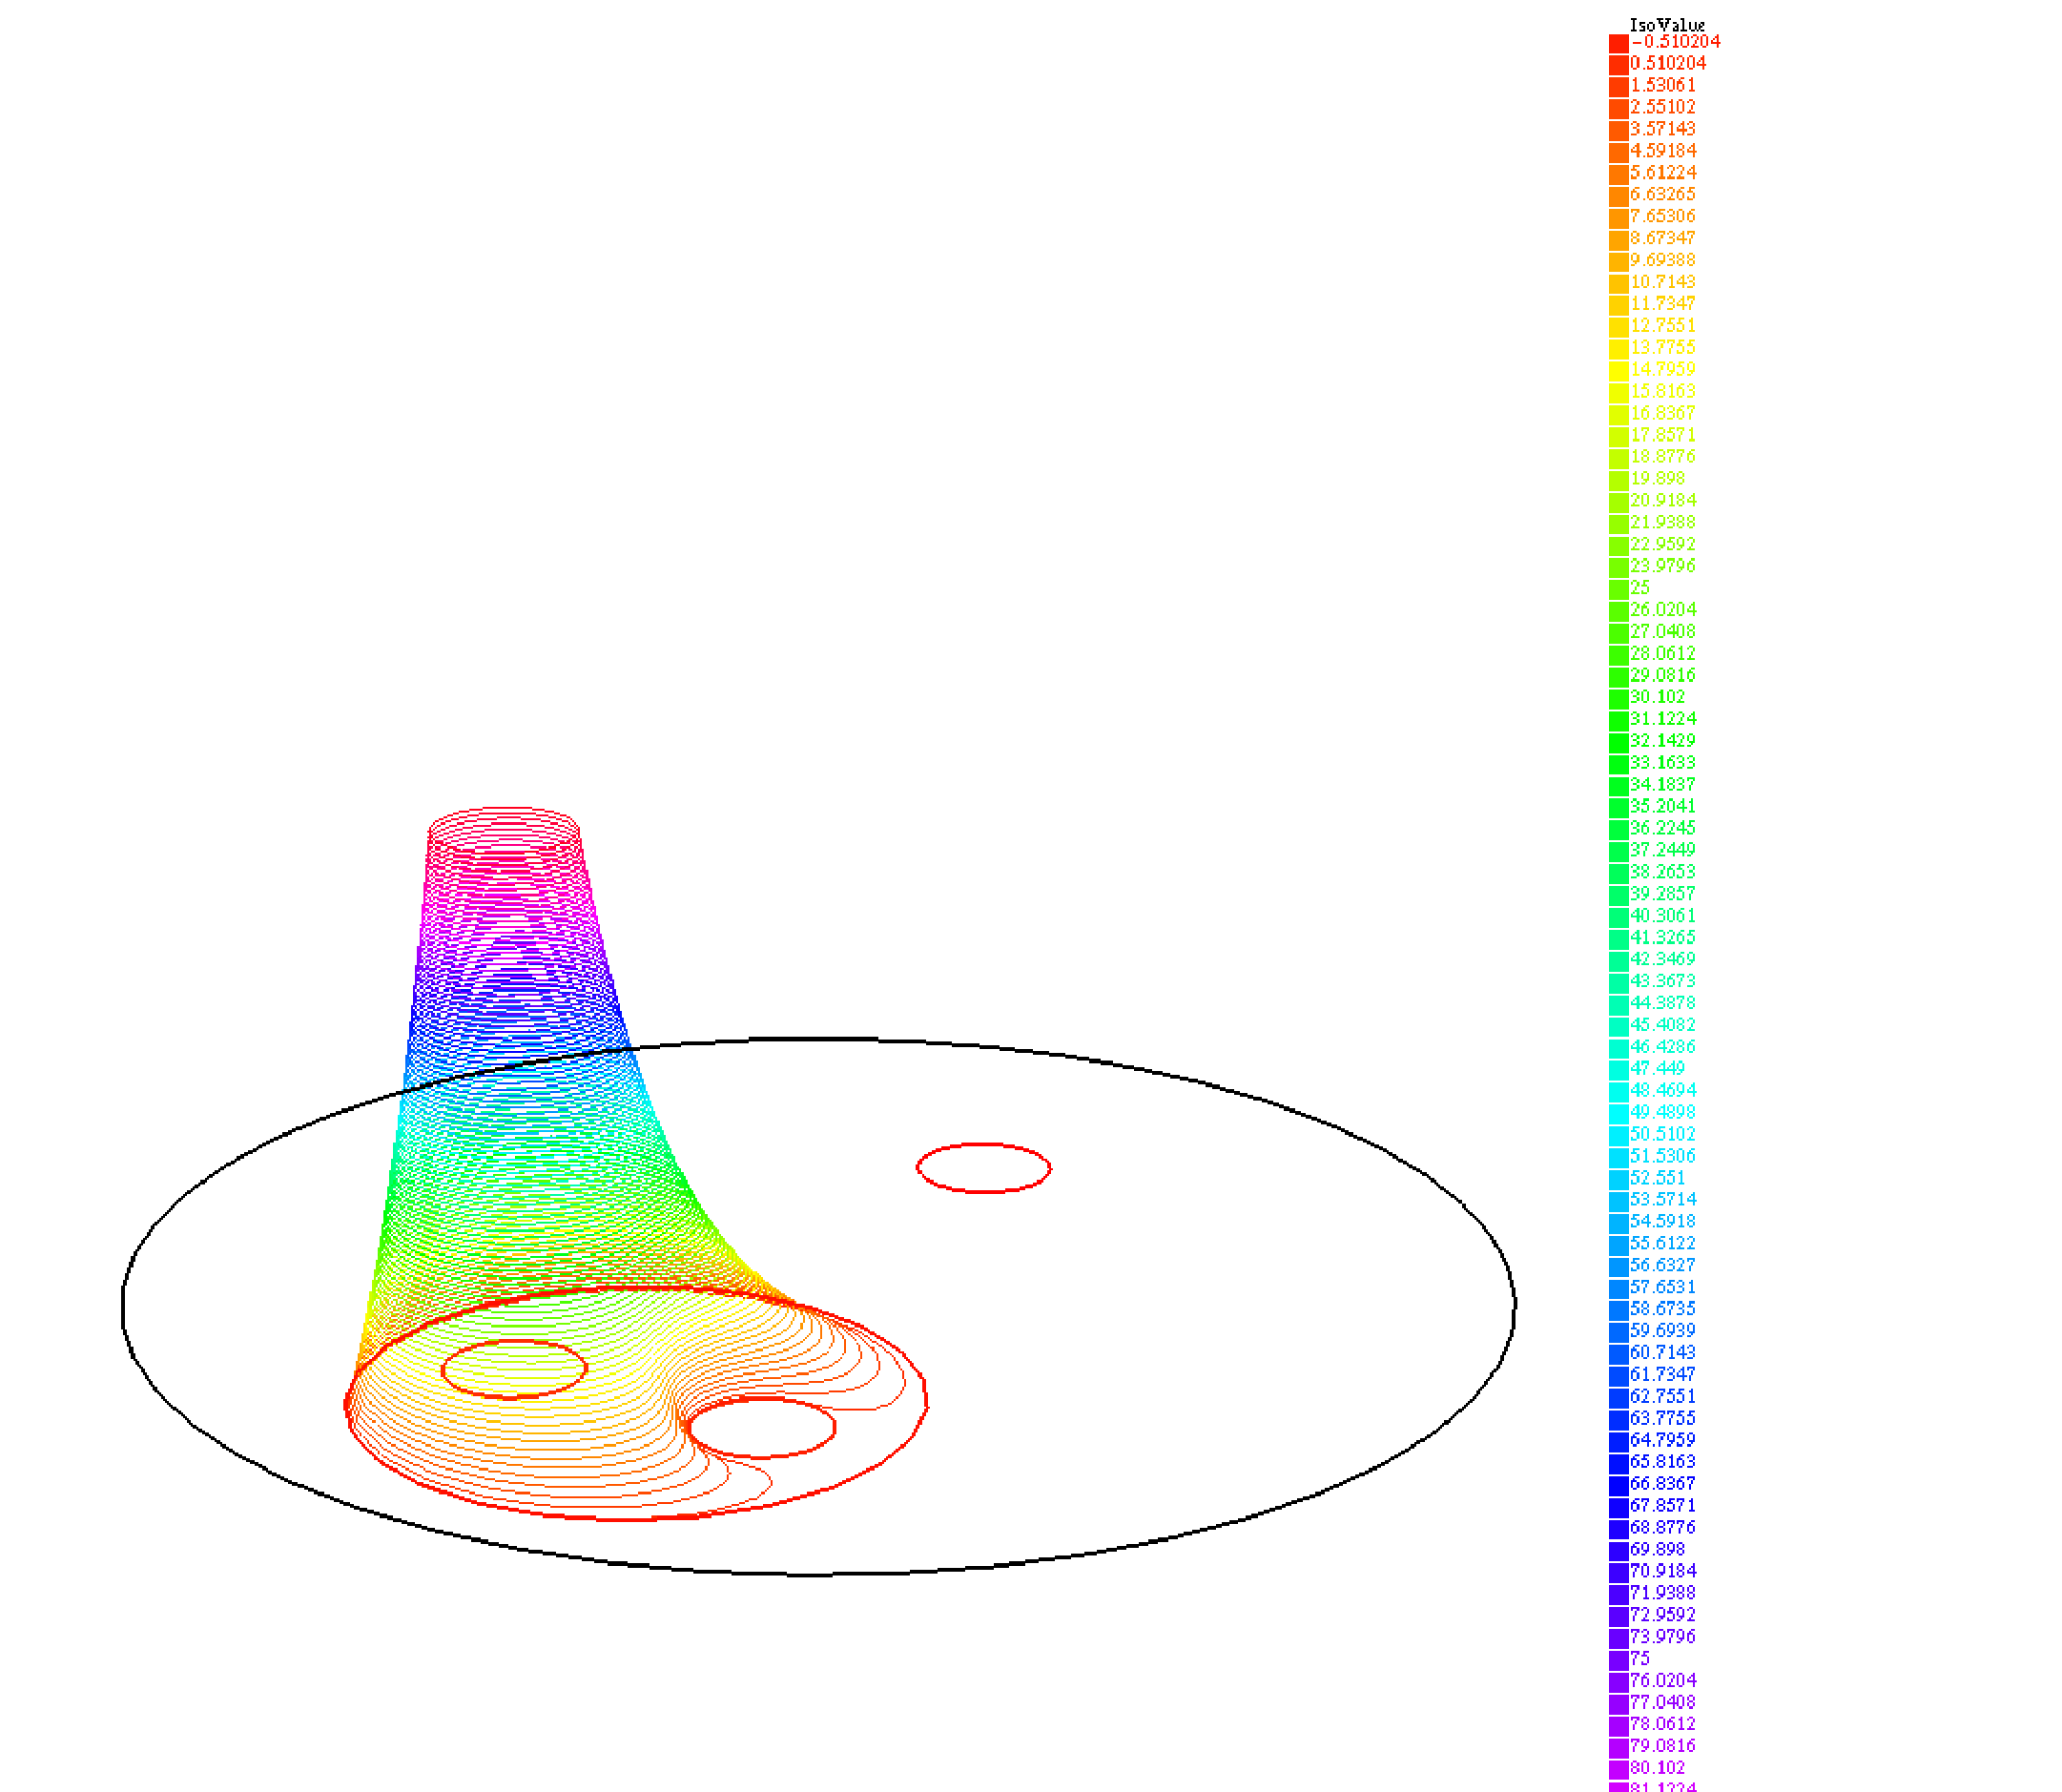
\includegraphics[width=.7\linewidth]{figures/gui/sol3D-1.pdf}
  \end{columns}
\end{frame}
%-------------------------------------------------------------------------------

%-------------------------------------------------------------------------------
\begin{frame}
    \frametitle{Maillage multi-niveaux}
    \begin{columns}[T]
        \column{.5\linewidth}
        \centering
        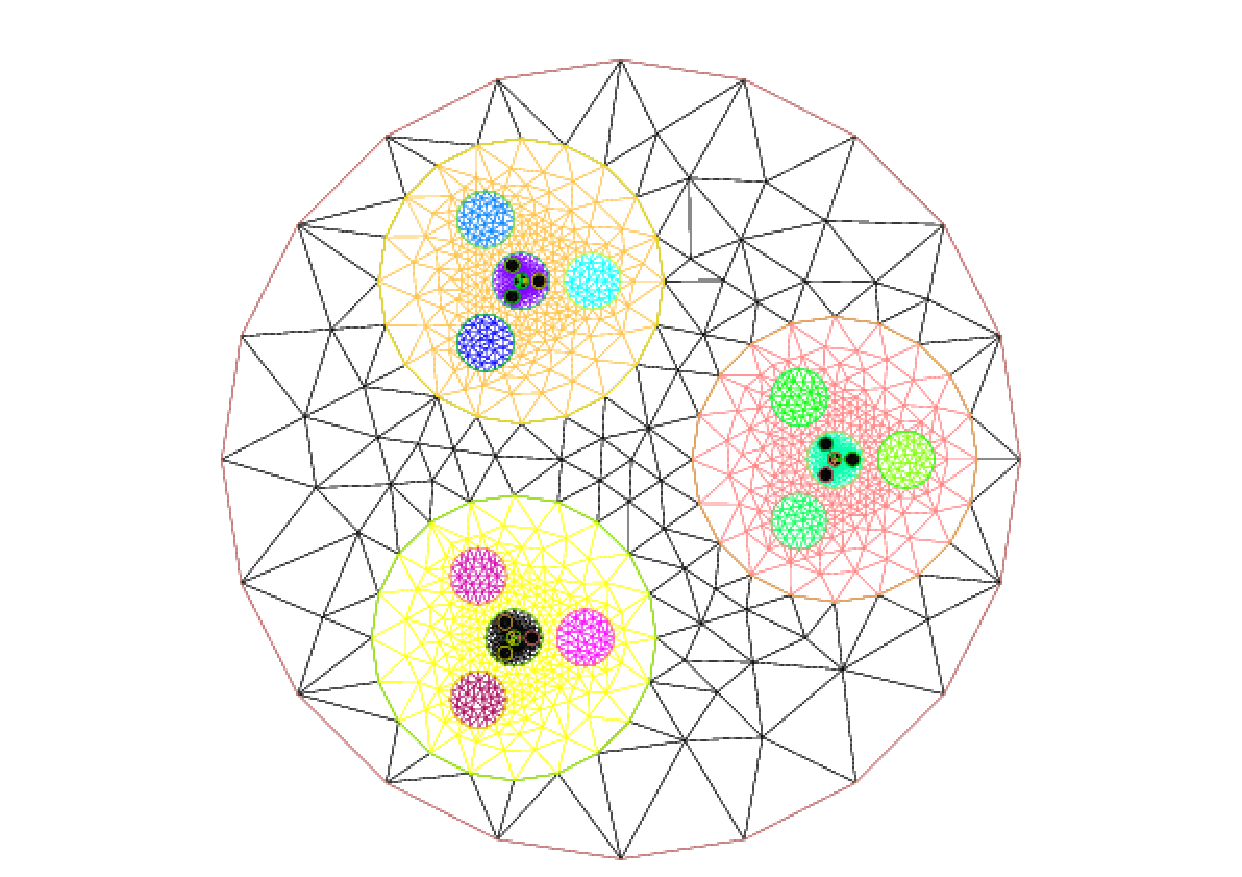
\includegraphics[width=1.2\linewidth]{figures/gui/mesh-2.pdf}
        \column{.5\linewidth}
        Création de différent niveaux de conducteurs par construction itérative:
        \begin{itemize}
            \item Blindage principale extérieur contenant 3 blindages
            \item Chaque sous blindage contient 3 conducteurs et 1 blindage
            \item Répétition des deux précédentes étapes dans les étages inférieurs
        \end{itemize}
    \end{columns}
    L'idée est de retrouver le défaut de positivité qui apparait sur ce genre de géométrie.
\end{frame}
%-------------------------------------------------------------------------------

%-------------------------------------------------------------------------------
\begin{frame}
  \frametitle{Comparaison et difficultés}
  \begin{columns}[T]
      \column{.5\linewidth}
  \begin{itemize}
      \item Découpez chaque niveau de maillage en sous maillage en respectant la numérotation.
      \item Dans le cas du découplage, chaque conducteur est considéré comme un trou sur la
          géométrie.
  \end{itemize}
      \column{.5\linewidth}
  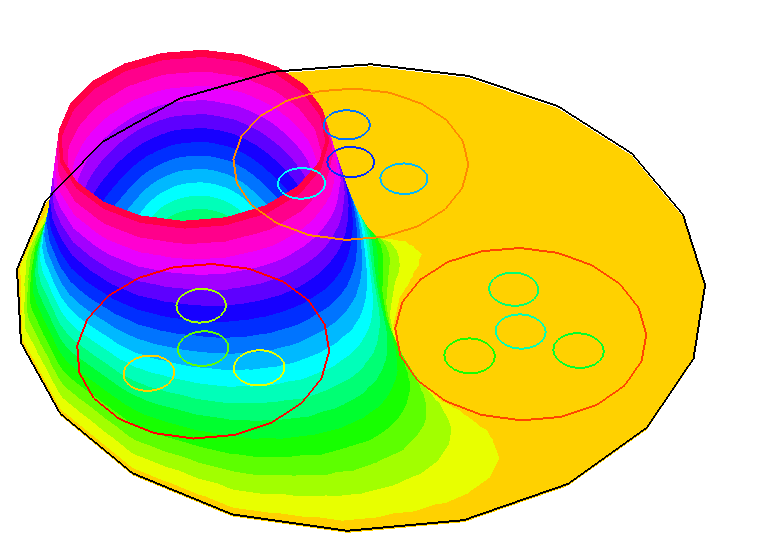
\includegraphics[width=.5\linewidth]{figures/gui/sol3Dfull2-1.png}
  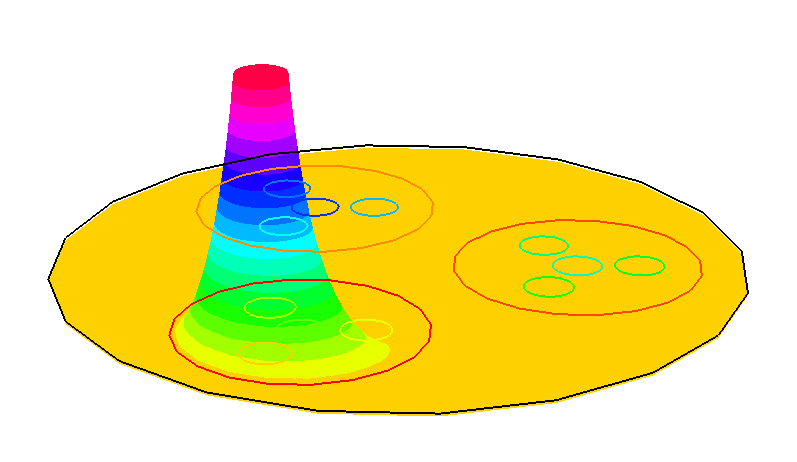
\includegraphics[width=.5\linewidth]{figures/gui/sol3Dfull2-2.png}\\
  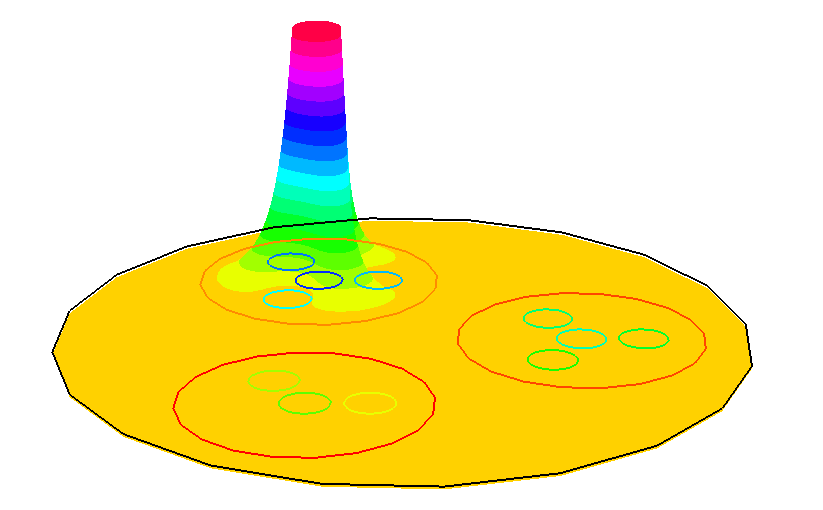
\includegraphics[width=.5\linewidth]{figures/gui/sol3Dfull2-3.png}
  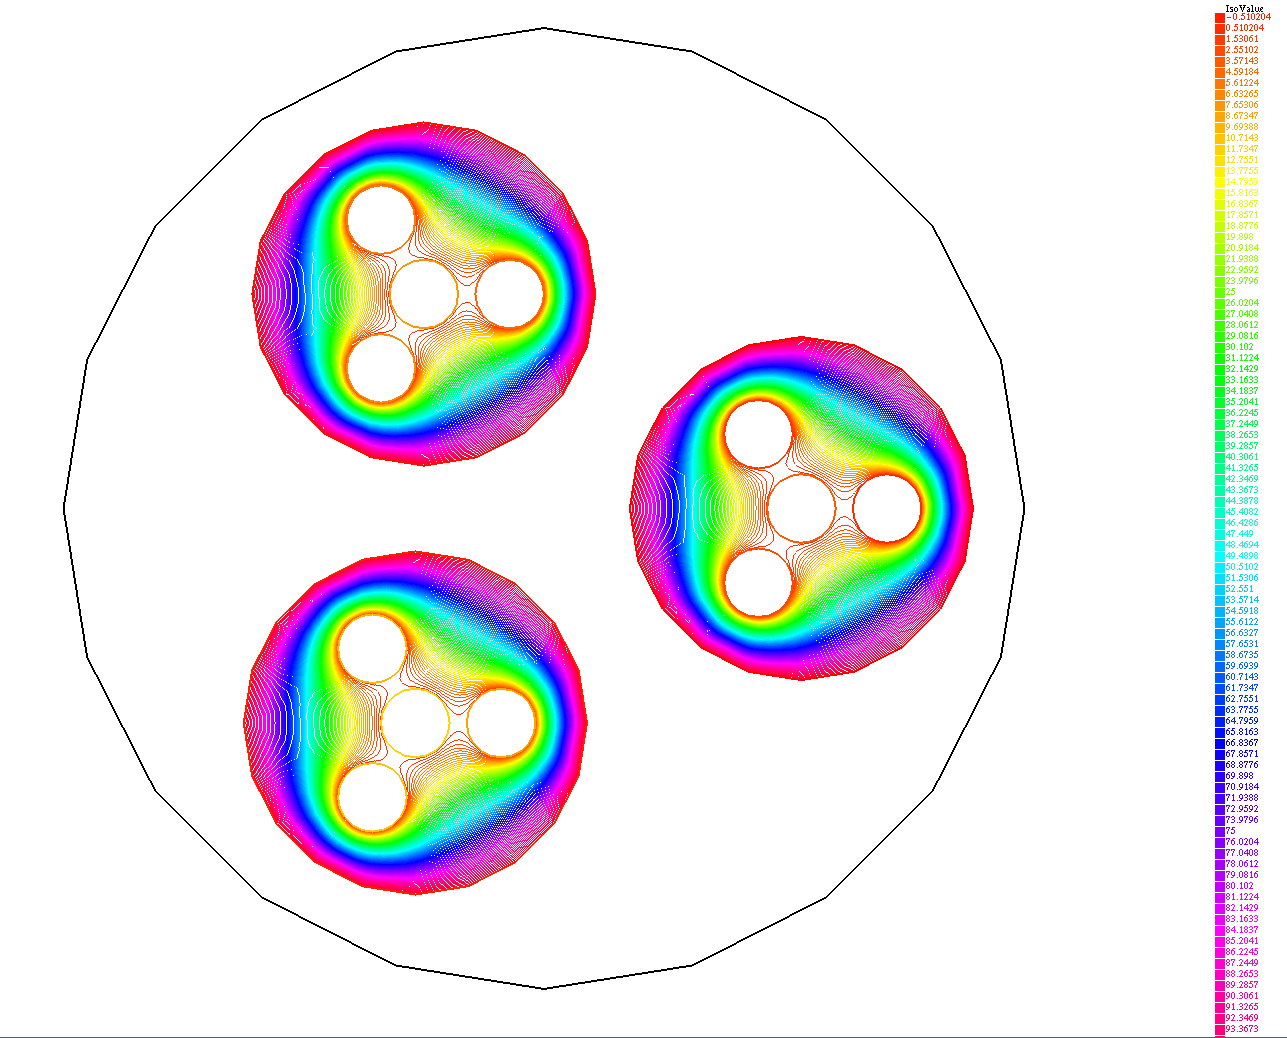
\includegraphics[width=.5\linewidth]{figures/gui/sol3Dfull2-4.png}
  \end{columns}
\end{frame}
%-------------------------------------------------------------------------------
